\chapter{问题描述}
\section{多目标检测与追踪问题描述}

给定图像序列${I_1, I_2,..., I_t}$, 每帧图像中有$M_t$个目标,其中t是当前帧号,每个目标的状态为$ s_1(t) $,其中状态一般包括位置,速度,加速度,朝向等。
\begin{equation}
	s_i(t) = \{ x,y,z,h,w,l,v_x,v_y,v_z,\theta \}
\end{equation}

当前帧的所有目标的状态就能表示成
\begin{equation}
	S(t) = \{ s_1(t), s_2(t),s_3(t),...,s_{M_t}(t) \}
\end{equation}

而每个目标的的轨迹则可以描述成
\begin{equation}
	s_i(1:t) = \{ s_i(1),s_i(2),s_i(3),...,s_i(t) \}
\end{equation}

则所有目标的状态集合就能表示成
\begin{equation}
	S(1:t) = \{ S_1. S_2,...S_t \}
\end{equation}

同理,我们类似的得到观测结果的定义,记作$ o_i(t),o_i(1:t),O(1:t) $。

而多目标跟踪任务就是通过观测结果找出所有目标的状态,我们用后验估计来进行描述。
\begin{equation}
	S(1:t) = argmax_{S(1:t)}P(S(1:t)|O(1:t))
\end{equation}

\section{问题的求解}
多目标检测与追踪一般的求解都基于TBD架构,如图\ref{dbt}所示。
\begin{figure}[H]
	\centering
	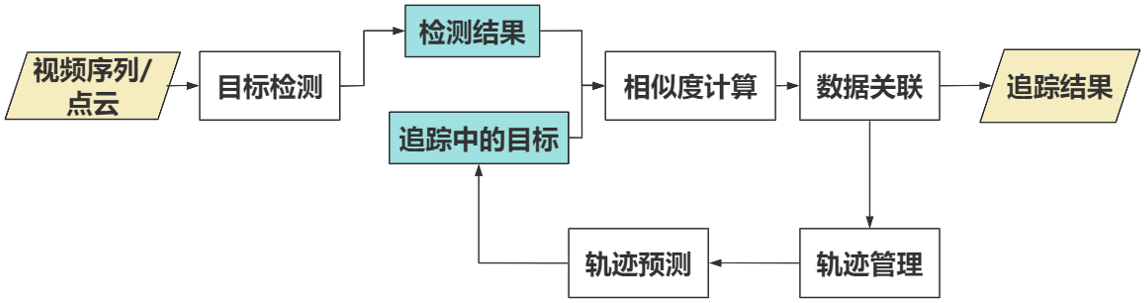
\includegraphics[width=\textwidth]{images/DBT.png}
	\caption{基于检测的追踪框架}
	\label{dbt}
\end{figure}


\section{滤波的作用}
主要概括,滤波的作用主要包括两个部分,融合多个传感器的追踪结果以及对目标进行预测,最终的目的都是为了得到更好的估计值。
它主要应用在图\ref{dbt}中轨迹预测部分。

\begin{tcolorbox}[]
	首先构建线性系统的状态空间描述:
	$$ \mathbf{x}_{t} = \mathbf{A} \mathbf{x}_{t-1} + \mathbf{B} \mathbf{u}_{t} + \bm{\epsilon}_{t} $$
	$$  \mathbf{z}_{t} = \mathbf{H} \mathbf{x}_{t} + \bm{\delta}_{t} $$
	
	接着利用卡尔曼滤波器进行最优状态估计:
	\begin{equation}
		\hat{\bm{x}}_{t}^{-} =  \bm{A} \hat{\bm{x}}_{t} + \bm{B} \bm{u}_t
	\end{equation}
	\begin{equation}
		\bm{\Sigma}_{t}^{-} = \bm{A} \bm{P}_{t-1} \bm{A}^{T} + \bm{Q}
	\end{equation}
	\begin{equation}
		\bm{K}_t = \frac{\bm{\Sigma}_{t}^{-} \bm{H}^{T}}{\bm{H} \bm{P}_{t}^{-} \bm{H}^{T} + \bm{R} }
	\end{equation}
	\begin{equation}
		\hat{\bm{x}}_t = \hat{\bm{x}}_{t-1} + \bm{K}_t(\bm{z}_t - \bm{H} \hat{\bm{x}}^{-})
	\end{equation}
	\begin{equation}
		\bm{P}_t = (\bm{I} - \bm{K}_t \bm{H}) \bm{P}_{t}^{-}
	\end{equation}
	
\end{tcolorbox}

\section{发展和思考}
1. \textbf{发展}

想要提高追踪的效果(精度,速度),可以从多个角度进行提高。大致可以包括几个方面:

仍旧基于BDT框架:追踪器的提升,数据融合方法的提升,数据关联的提升,滤波器的提升(包括模型改进)。

新的框架:端到端\cite{10610979},基于点的移动的追踪\cite{wu2024moving}。

2. \textbf{思考}

首先确定融合的框架:DBT和神经网络融合结构。
接着确定数据关联方式,倾向于用特征值(点)
然后改进滤波器的结构:模型的改进(长时间拟合),噪声的优化(A-KIT)
最后,连接最新的检测器。

实际实验:标定,ROS表示


\chapter{DeepVO: Towards End-to-End Visual Odometry with Deep Recurrent Convolutional Neural Networks"\cite{wang_deepvo_nodate}}

\section{问题描述}

DeepVO首次提出了一种端到端的视觉里程计算法,整个流程只需要给视频就能够得到状态。其将状态估计问题描述成一个最大似然估计问题。

\begin{tcolorbox}[]
	对于给定的单目相机图片序列,计算姿态的条件概率。
	
	$$P(Y_t|X_t) = (y_1,y_2,...y_t|x_1,x_2,...x_t)$$
	
	利用神经网络进行建模之后,问题就成为求解网络最优超参数$\theta^*$的问题:
	
	$$\theta^{*} = \arg\max_{\theta} p(Y_{t}|X_{t}; \theta)$$
\end{tcolorbox}

\section{解决方法}
第一次提出了用端到端的方法求解状态估计问题,其具体网络结构如图\ref{deepvo1}所示。

\begin{figure}[H]
	\centering
	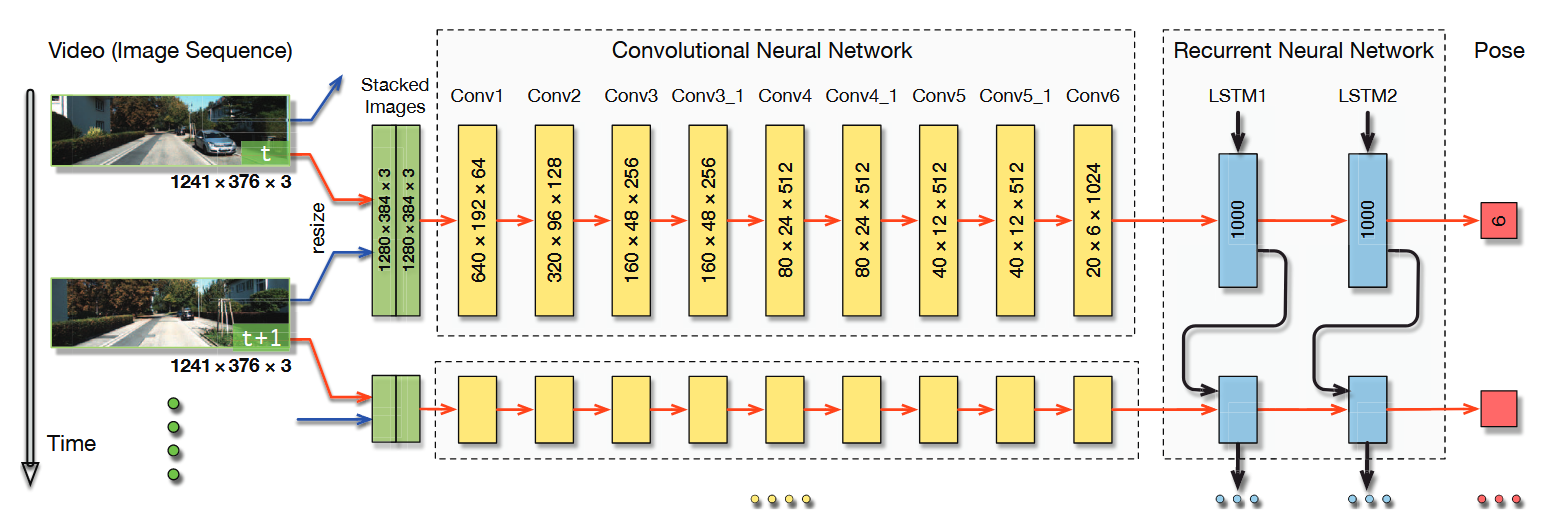
\includegraphics[width=\textwidth]{images/deepvo1.png}
	\caption{DeepVO整体网络结构}
	\label{deepvo1}
\end{figure}

其中的RNN结构部分,考虑到了物体的运动方程,在潜状态空间进行了建模,其节点结果如图\ref{rnn_point}所示。
\begin{figure}[H]
	\centering
	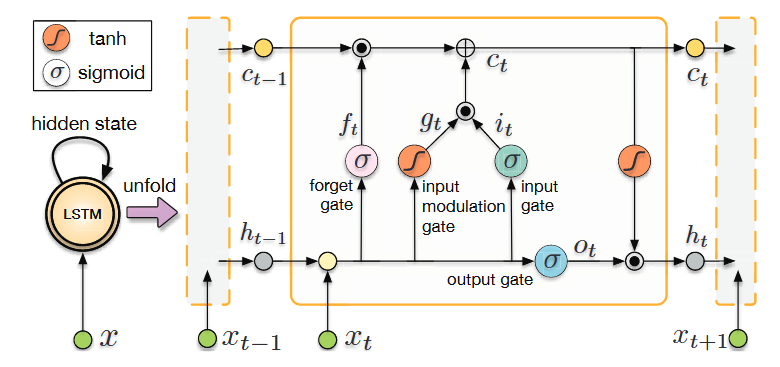
\includegraphics[width=0.8\textwidth]{images/deepvo/rnn_point.png}
	\caption{RNN节点结构}
	\label{rnn_point}
\end{figure}

其构建的模型:
\begin{figure}[H]
	\centering
	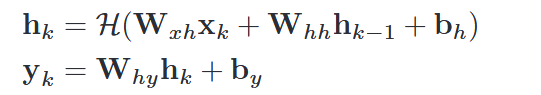
\includegraphics[width=0.5\textwidth]{images/deepvo/fuc1.png}
\end{figure}

其具体内部的参数计算则是:
\begin{figure}[H]
	\centering
	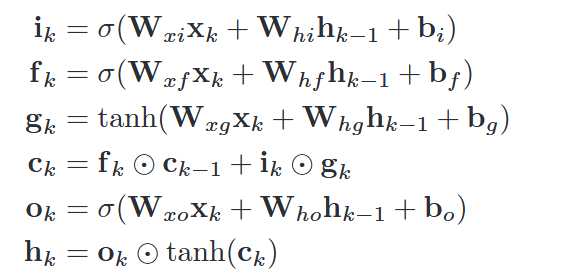
\includegraphics[width=0.5\textwidth]{images/deepvo/fuc2.png}
\end{figure}

其中主要的参数说明:$h_k$是潜状态,$x_k$是输入的图像,$y_k$是输出的姿态,$c_k$是记忆存储单元(记录了之前的运算结果),$W_k$是网络权重。

\section{仿真结果}

\begin{figure}[H]
	\centering
	
	% 第一排
	\begin{minipage}{0.45\textwidth}
		\centering
		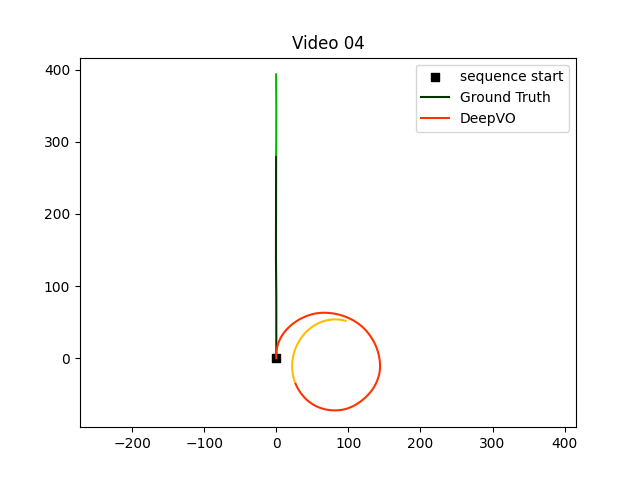
\includegraphics[width=\textwidth]{images/DeepVO/route_04_gradient.png}
		\caption{序列4测试结果}
		\label{fig:deepvo:4}
	\end{minipage}
	\hfill
	\begin{minipage}{0.45\textwidth}
		\centering
		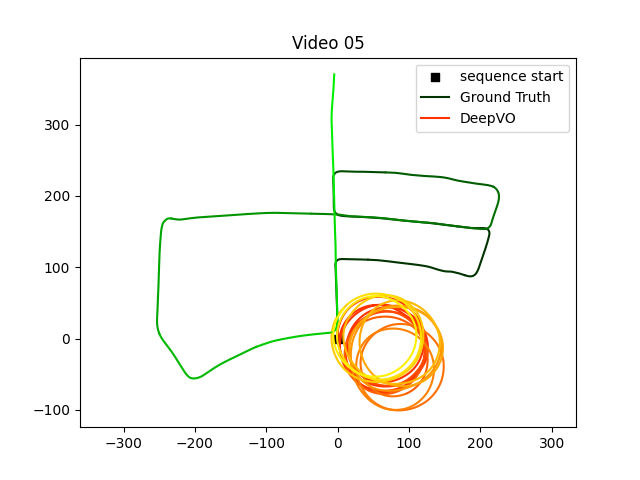
\includegraphics[width=\textwidth]{images/DeepVO/route_05_gradient.png}
		\caption{序列5测试结果}
		\label{fig:deepvo:5}
	\end{minipage}
	
	% 第二排
	\vskip\baselineskip % 垂直间隔,可以根据需要调整
	
	\begin{minipage}{0.45\textwidth}
		\centering
		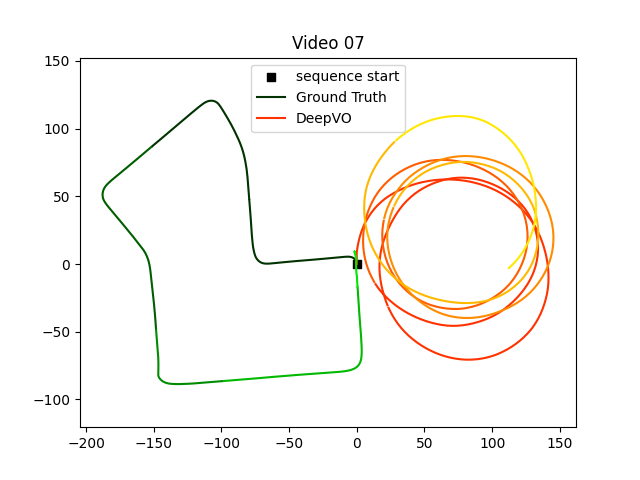
\includegraphics[width=\textwidth]{images/DeepVO/route_07_gradient.png}
		\caption{序列7测试结果}
		\label{fig:deepvo:7}
	\end{minipage}
	\hfill
	\begin{minipage}{0.45\textwidth}
		\centering
		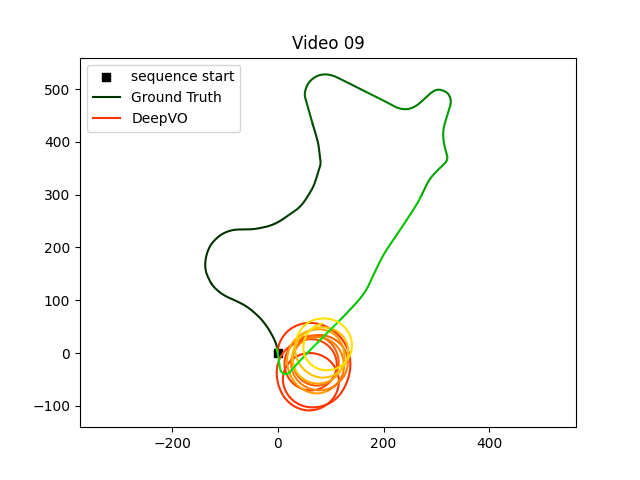
\includegraphics[width=\textwidth]{images/DeepVO/route_09_gradient.png} 	
		\caption{序列9测试结果}
		\label{fig:deepvo:9}
	\end{minipage}
	
	% 第三排(如果第五张图片需要单独一行,可以省略下面的 minipage 对)
	% \vskip\baselineskip % 如果需要额外的垂直间隔
	
	% \begin{minipage}{0.45\textwidth}
		%     \centering
		%     \includegraphics[width=0.9\textwidth]{image5.png} % 可以调整宽度以适应单独一行
		%     \caption{Image 5}
		%     \label{fig:image5}
		% \end{minipage}
	% \hfill
	% \begin{minipage}{0.45\textwidth}
		%     \centering
		%     % 空白 minipage 以保持布局对齐
		% \end{minipage}
	
	% 或者,如果第五张图片直接放在下一行,不需要 minipage 对齐
	\vskip\baselineskip % 如果需要额外的垂直间隔
	\centering
	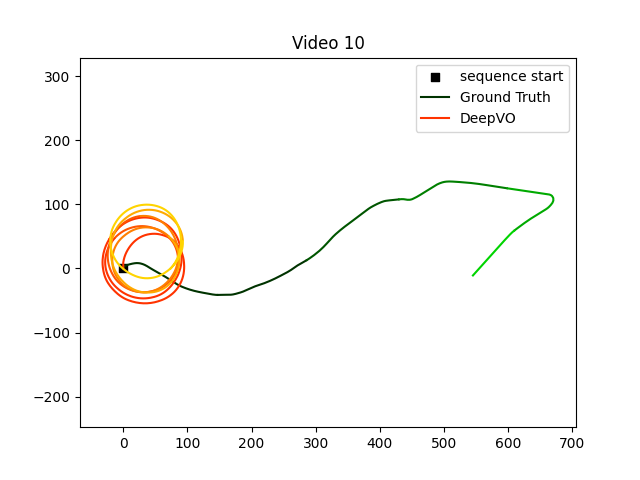
\includegraphics[width=0.45\textwidth]{images/DeepVO/route_10_gradient.png}
	\caption{序列10测试结果}
	\label{fig:deepvo:10}
	
\end{figure}


\section{学习体会}

DeepVO首次提出了一种端到端的视觉里程计算法,整个流程只需要给视频就能够得到状态。最终的效果还算不错(并没有完全取代传统方法)。
试着运行了端到端算法的效果,作为以后对比的内容。

可以发现纯神经网络算法的效果并没有达到最优,而且存在数据集不足,应对场景泛化能力不足,原理黑盒等问题。但是他们也展现出一些优势:不需要进行复杂的建模,整体的结构简单容易实现。




\chapter{论文“SWformer-VO: A Monocular Visual Odometry Model Based on Swin Transformer”\cite{swformer}学习}
\section{问题描述}
本文是对之前基于学习的方法的改进,问题描述同DeepVO。
基于学习的方法距离效果最好的视觉里程计还有一定的差距。此外,一些新的学习方法的计算复杂度比较高。

\section{解决方法}
1. 将swim-transformer结构应用到视觉里程计的任务上,据此计算复杂度由二次方降低为线性,大大提高了计算效率。提出的网络结构如图\ref{fig:sw:1}所示。

\begin{figure}[htbp]
	\centering
	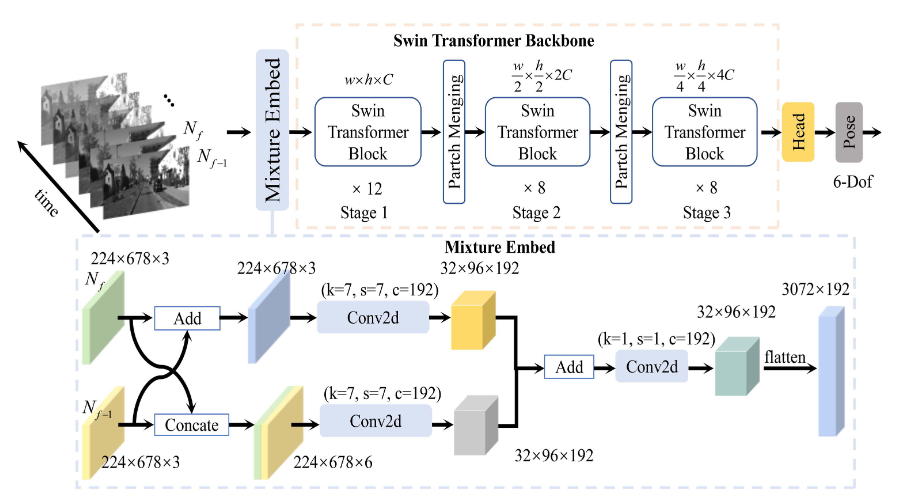
\includegraphics[width=0.8\textwidth]{images/swformer/swformer.png}
	\caption{swformer网络结构}
	\label{fig:sw:1}
\end{figure}

新网络的计算复杂度和过去基于Transformer网络的方法相比显著下降。

\begin{figure}[H]
	\centering
	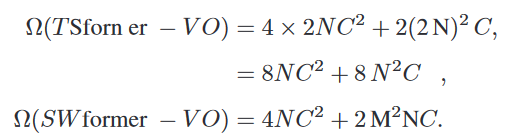
\includegraphics[width=0.5\textwidth]{images/swformer/swformer_compute.png}
	\caption{计算复杂度的降低}
	\label{fig:sw:2}
\end{figure}

2. 提出了一种“Mixture Embed Module”模块对图像进行预处理,由此构成网络。

文受启发于“视觉残留”现象,提出了一种帧间插值的方法,如图\ref{fig:sw:1}所示。这种方法顺利的减小了计算量,由原来需要处理连续的两帧图片,变成了处理一个经过预处理的合成图片。

\section{代码复现}
1. 训练

训练了50轮次
\begin{figure}[htbp]
	\centering
	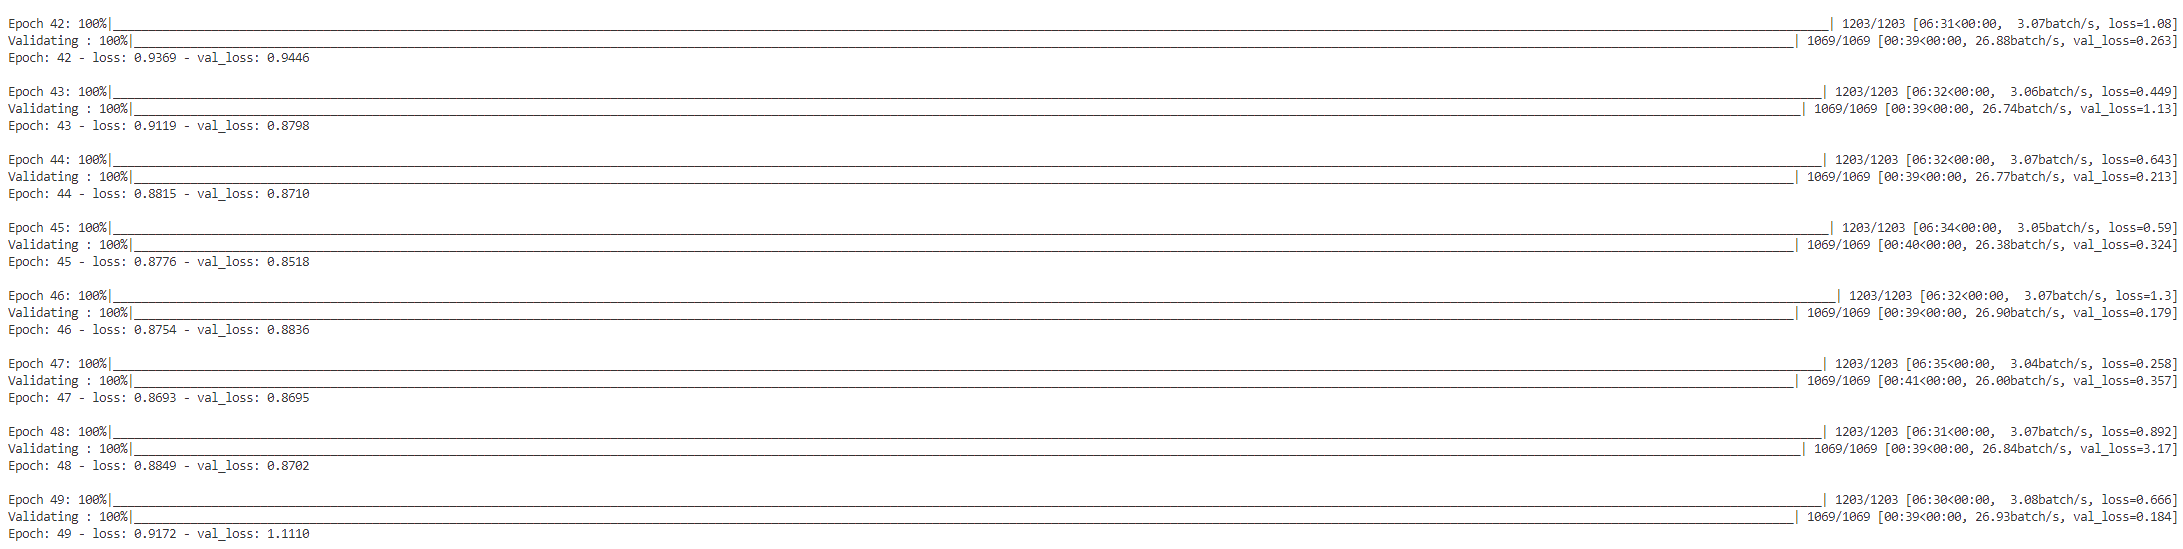
\includegraphics[width=\textwidth]{images/swformer/train.png}
	\caption{网络训练结果}
	\label{fig:sw:3}
\end{figure}

2. 测试
如图\ref{fig:swformer:08}、\ref{fig:swformer:09}、\ref{fig:swformer:10}所示。

\begin{figure}[H]
	\centering
	
	% 第一排
	\begin{minipage}{0.45\textwidth}
		\centering
		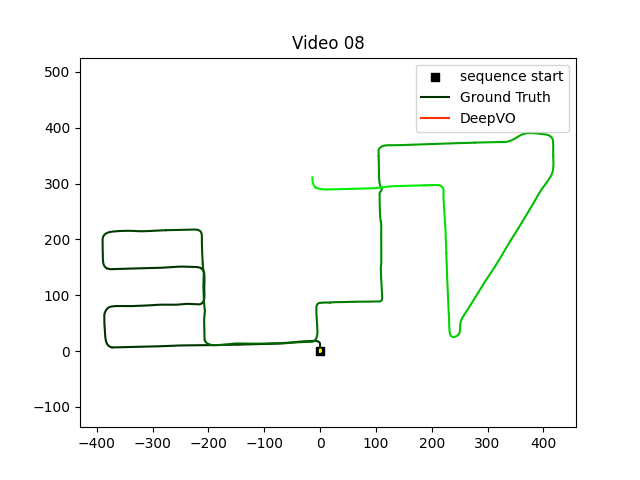
\includegraphics[width=\textwidth]{images/swformer/route_08_gradient.png}
		\caption{序列8测试结果}
		\label{fig:swformer:08}
	\end{minipage}
	\hfill
	\begin{minipage}{0.45\textwidth}
		\centering
		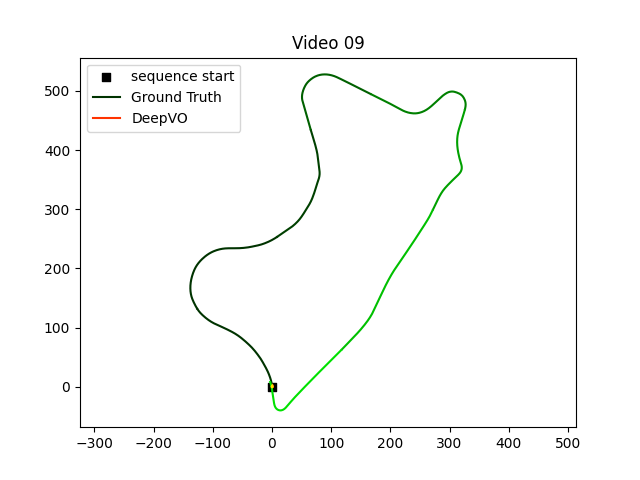
\includegraphics[width=\textwidth]{images/swformer/route_09_gradient.png}
		\caption{序列9测试结果}
		\label{fig:swformer:09}
	\end{minipage}
	
	\vskip\baselineskip % 如果需要额外的垂直间隔
	\centering
	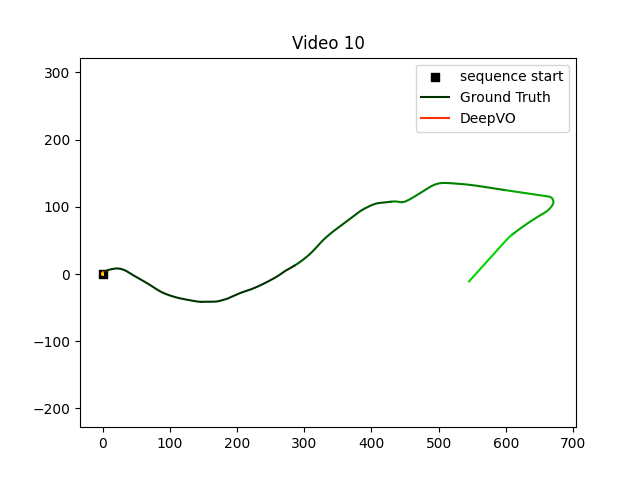
\includegraphics[width=0.45\textwidth]{images/swformer/route_10_gradient.png}
	\caption{序列10测试结果}
	\label{fig:swformer:10}
	
\end{figure}

\section{总结与思考}
虽然该论文也是端到端的学习算法,不过依旧可以从中学到一些内容。

1. 数据集的补充

根据阅读的两篇论文,我发现它们都提到了数据集的不足。学习类的算法是非常依赖数据集的数量和质量的,本文再次映证了这一点。

2. swim-transformer结构的学习

transformer的实际应用需要进行一定的本地化,因此学界提出了swim-transformer的结构。后面需要仔细了解这以结构的原理和实现。

3. 图像预处理技术

由于需要处理运动学的问题,那么我们就需要在一个时刻内处理多帧图像。本文就提供了一种处理方法。
